\newcommand*{\Cr}{\mathrm C}
\newcommand*{\rs}{\mathrm r}
\newcommand*{\st}{\mathrm s}

\chapter{系综}

前面讨论的是近独立粒子系统,忽略粒子间作用,用单粒子态分布描述系统状态;如果粒子间作用不能忽略,单粒子态无确切含义,就要以系统为整体研究,这就是\textbf{系综}。系综的平均值就是统计平均值。

\section{系统微观状态的描述与统计系综}

经典理论中,粒子状态由广义坐标$q$与广义动量$p$描述,张成$\mu$空间。而系统的微观状态由$\varGamma$空间描述
\begin{definition}{$\varGamma$空间}{Gamma Space}
	$\varGamma$空间是所有粒子广义坐标$q_i$与广义动量$p_i$所张的空间,相体积元
	\begin{align}
		\d\Omega=\prod_{i=1}^f\d q_i\nd p_i,
	\end{align}
	其中$f=N\gamma$为整个系统的自由度。
\end{definition}

用$\rho(q,p,t)$表示系统在时刻$t$处于相体积元$\d\Omega$的几率,$\rho(q,p,t)$称为分布函数,满足归一化条件
\[
	\int_\varGamma\rho(q,p,t)\d\Omega=1.
\]
宏观量是各微观态对应量$B(q,p)$的统计平均值
\begin{equation}
	\avg B(t)=\int_\varGamma B(q,p)\rho(q,p,t)\d\Omega.
\end{equation}

\begin{theorem}
	{Liouville定理}{Liouville Theorem}
	孤立系统在$\varGamma$空间中运动时,其分布函数$\rho(q,p,t)$满足Liouville方程
	\begin{equation}
		\dv\rho t=\pv\rho t+\sum_{i=1}^f\kh{\pv\rho{q_i}\pv H{p_i}-\pv\rho{p_i}\pv H{q_i}}=0.
	\end{equation}
\end{theorem}

% \begin{proof}
% 	$\rho$的微分为
% 	\[
% 		\d\rho=\pv\rho t\d t+\sum_{i=1}^f\biggkh{\pv\rho{q_i}\d q_i+\pv\rho{p_i}\d p_i},
% 	\]
% 	由Hamilton方程
% 	\[
% 		\dv{q_i}t=\pv H{p_i},\quad \dv{p_i}t=-\pv H{q_i},
% 	\]
% 	即证。
% \end{proof}

量子中,系统微观状态用力学量完全集的量子数描述,由不确定度关系,每个量子态在$\varGamma$空间占据相体积$h^f$。

\begin{definition}{系综}{ensemble}
	系综(ensemble)是大量微观结构、宏观条件相同的系统的集合。
	\begin{compactitem}
		\item 微正则系综(micro canonical ensemble):孤立系统,$N,V,U$恒定;
		\item 正则系综(canonical ensemble):封闭系统,$N,V,T$恒定;
		\item 巨正则系综(grand canonical ensemble):开放系统,$\mu,V,T$恒定。
	\end{compactitem}
\end{definition}
后面会看到,在粒子数$N\to\infty$且$N/V$恒定时,三个系综等价。
\section{微正则分布}
平衡的孤立系统服从的分布叫微正则分布。满足Boltzmann等几率假设:处平衡态的孤立系统,各可能微观状态出现的几率相等。

微正则系综的特性函数就是熵
\[
	\rho_\st=\frac1\Omega,\quad S=-\sum_\st\rho_\st\ln\rho_\st.
\]
\section{正则分布}
考虑系统$A$与热源$A_\rs$间的平衡,注意到$A+A_\rs$构成孤立系统,当二者相互作用可忽略时,总能量$E^{(0)}=E_\st+E_\rs$,且对很大的热源$E_\rs\gg E_\st$。记当$A$处于系统$E_\st$某一量子态,$A_\rs$处于系统$E_\rs$任一量子态,微观态数目为$\Omega_\rs(E_\rs)$
\[
	\ln\Omega_\rs(E_\rs)=\ln\Omega_\rs(E^{(0)}-E_\st)\simeq\ln\Omega_\rs(E^{(0)})-\beta E_\st
\]
故分布概率
\[
	\rho_\st\propto\e{-\beta E_\st}\xrightarrow{\text{normalize}}\rho_\st=Z^{-1}\e{-\beta E_\st}.
\]
配分函数
\[
	Z=\sum_\st\e{-\beta E_\st}.
\]
由定义,$\beta$只与热源有关,不同系统达到平衡时温度相同,故$\beta=\beta(T)$。

若能级有简并度$\varGamma_\st$,则 
\begin{align}
	Z=\sum_\st\varGamma_\st\e{-\beta E_\st}.
\end{align}
\paragraph{正则分布的热力学公式}内能
\begin{align}
	E=\sum_\st\rho_\st E_\st=Z^{-1}\sum_\st E_\st\e{-\beta E_\st}=-\pv{\ln Z}\beta.
\end{align}
状态方程
\begin{align}
	Y_i=\sum_\st\rho_\st\pv{E_\st}{y_i}=-\frac1\beta\pv{\ln Z}{y_i}.
\end{align}
熵
\begin{align*}
	T\d S&=\d E-\sum_i Y_i\d y_i=-\d\kh{\pv{\ln Z}\beta}+\frac1\beta\sum_i\pv{\ln Z}{y_i}\d y_i\\
	&=-\d\kh{\pv{\ln Z}\beta}+\frac1\beta\fkh{\d(\ln Z)-\pv{\ln Z}\beta\d\beta}\\
	&=\frac1\beta\d\kh{\ln Z-\beta\pv{\ln Z}\beta}.
\end{align*}
两边全微分要求$\kB T=\beta$,且 
\begin{align}
	S-S'=\kB\kh{\ln Z-\beta\pv{\ln Z}\beta}=\kB(\ln Z+\beta E).
\end{align}

另一方面,由Boltzmann关系
\begin{align*}
	S&=\kB\ln\Omega\{M_\st\}=\kB\kh{\ln M!-\sum_\st\ln M_\st!}\\
	&\simeq\kB\fkh{M(\ln M-1)-\sum_\st M_\st(\ln M_\st-1)}
\end{align*}
而
\[
	\ln M_\st=\ln M-\ln Z-\beta E_\st
\]
故$S'=0$。

从微观角度说,
\begin{align}
	S=-\kB\sum_\st\rho_\st\ln\rho_\st.
\end{align}
自由能
\begin{align}
	F=E-TS=-\kB T\ln Z.
\end{align}
\paragraph{能量涨落}由
\begin{align*}
	\ave{E^2}&=\sum_\st\rho_\st E_\st^2=Z^{-1}\sum_\st E_\st^2\e{-\beta E_\st}\\
	&=Z^{-1}\pv[2]Z\beta=\pv[2]{\ln Z}\beta+\kh{\pv{\ln Z}\beta}^2\\
	&=\kB T^2C_V+\ave E^2
\end{align*}
能量的绝对涨落
\begin{align}
	\D E^2=\ave{E^2}-\ave E^2=\kB T^2C_V.
\end{align}
\begin{example}{单原子分子理想气体的相对涨落}{}
	能量$E=\frac32 N\kB T$,比热$C_V=\frac32N\kB$,故相对涨落
	\[
		\vd E=\frac{\D E}E=\sqrt{\frac2{3N}}\sim 10^{-11}
	\]
	涨落对宏观系统量很小的。
\end{example}
因而,$E$可看作是孤立系统的能量,用正则分布研究孤立系统。
\paragraph{正则分布的连续形式}$\varGamma$空间中,若能量准连续
\begin{align}
	Z=\frac1{N!}\frac1{h^f}\int\e{-\beta E}\prod_{i=1}^N\d q_i\nd p_i
\end{align}
能量曲面$H(p,q,y)=E$包围的相体积
\begin{align}
	\Omega(E)=\int_{H\leqslant E}\prod_{i=1}^N\d q_i\nd p_i.
\end{align}
故按能量分布
\begin{align}
	Z=\frac1{N!}\frac1{h^f}\int\zti\Omega'(E)\e{-\beta E}\d E.
\end{align}
\begin{example}{用正则分布求单原子理想气体状态方程}{}
	$N$个单原子分子气体的Hamilton量
	\[
		H=\sum_{i=1}^{3N}\frac{p_i^2}{2m}.
	\]
	则
	\[
		\Omega(E)=\int\d q\int_{H\leqslant E}\d p=V^N\cdot\frac{\pi^{3N/2}}{\kh{\frac{3N}2}!}(2mE)^{3N/2}.
	\]
	故
	\begin{align*}
		Z&=\frac1{N!h^{3N}}\int\zti\Omega'(E)\e{-\beta E}\d E\\
		&=\frac{V^N}{N!\kh{\frac{3N}2}!}\kh{\frac{2\pi m}{h^2}}^{3N/2}\cdot\frac{3N}2\int\zti E^{3N/2-1}\e{-\beta E}\d E\\
		&%=\frac{V^N}{N!\kh{\frac{3N}2}!}\kh{\frac{2\pi m}{h^2}}^{3N/2}\cdot\frac{3N}2\beta^{-3N/2}\Gamma\kh{\frac{3N}2}
		=\frac{V^N}{N!}\kh{\frac{2\pi m}{h^2\beta}}^{3N/2}=\frac{Z_\tl^N}{N!}.
	\end{align*}
	内能
	\begin{align}
		E=-\pv{\ln Z}\beta=\frac{3N}{2\beta}=\frac32N\kB T.
	\end{align}
	状态方程
	\begin{align}
		p=\frac1\beta\pv{\ln Z}V=\frac N{\beta V}=\frac{N\kB T}V.
	\end{align}
\end{example}
\section[实际气体的状态方程]{实际气体(非理想气体)的状态方程}
$N$个全同粒子,体积$V$,
\[
	E=E_\tl+\varPhi+E_\i.
\]
其中$E_\tl(p)$与质心平动有关,$\varPhi(q)$是分子间势能,$E_\i$是分子内部运动。故
\[
	Z=\frac1{N!h^{3N}}\int\e{-\beta E_\tl}\d p\int\e{-\beta\varPhi}\d q\cdot Z_\i.
\]
考虑分子间势能项
\[
	Q:=\int\e{-\beta\varPhi}\d q
\]
只考虑分子间两两相互作用,其作用势$\phi_{ij}\equiv\phi(r_{ij})$只与分子间距离有关,
\[
	\varPhi=\sum_{i<j}\phi_{ij}
\]
引入
\[
	f_{ij}=\e{-\beta\phi_{ij}}-1=
	\begin{cases}
		0,&r_{ij}\to\infty\\
		-1,&r_{ij}\to0
	\end{cases}
\]
分子作用力是短程的,故一般$\abs{f_{ij}}<1$,可展开
\[
	Q=\int\prod_{i<j}(1+f_{ij})\d q=\int\fkh{1+\sum_{i<j}f_{ij}+\frac12\overset{(i,j)\neq(k,\ell)}{\sum_{i<j}\sum_{k<\ell}}f_{ij}f_{k\ell}+\cdots}\d q.
\]
第三项后仅当多个分子都很接近时才显著,故只保留前两项
\[
	Q\simeq V^N+\frac12N(N-1)V^{N-2}\int f(r_{12})\d\bm r_1\nd\bm r_2.
\]
引入质心坐标$\bm R=\frac{m_1\bm r_1+m_2\bm r_2}{m_1+m_2}$和相对位置$\bm r=\bm r_1-\bm r_2$,易证$\det J=1$
\[
	\int f(r_{12})\d\bm r_1\nd\bm r_2=\int f(r)\d\bm r\nd\bm R=-2Va_2(T).
\]
第二级Virial系数
\begin{align}
	a_2(T)=-\frac12\int f(r)\d\bm r=-2\pi\int\zti\kh{\e{-\beta\phi(r)}-1}r^2\d r
\end{align}
故
\[
	Q\simeq V^N-N(N-1)V^{N-1}a_2(T)\simeq V^N\fkh{1-\frac{N^2}Va_2(T)}.
\]
取对数\footnote{过程中一系列近似相当于
\[
	\ln\e{-x}=\ln\kh{1-x+\frac12x^2+\cdots}\simeq\ln(1-x)\simeq -x
\]
即结果并不会不严格。}
\begin{align}
	\ln Q=N\ln V+\ln\fkh{1-\frac{N^2}Va_2(T)}\simeq N\ln V-\frac{N^2}Va_2(T).
\end{align}
状态方程
\begin{align*}
	p=\frac1\beta\pv{\ln Q}V=\frac1\beta\fkh{\frac NV+\frac{N^2}{V^2}a_2(T)}.
\end{align*}
故
\begin{align}
	\frac{pv}{\kB T}=1+\frac{a_2(T)}v.
\end{align}
\begin{example}{Van der Waals力}{Van der Waals Force}
	1930年London证明瞬时电偶极矩之间力
	\begin{equation}
		\phi(r)=\phi_0\fkh{\kh{\frac{r_0}r}^{12}-2\kh{\frac{r_0}r}^6}\simeq\begin{cases}
			\infty,&r<r_0\\
			-\phi_0\kh{\frac{r_0}r}^6,&r>r_0
		\end{cases}
	\end{equation}
	\begin{center}
		\includegraphics[page=25]{figures/tikz/coordinates.pdf}
		\captionof{figure}{$\phi\vs r$图像}
		\label{fig:phi(r)}
	\end{center}
	故
	{\begin{align*}
		a_2(T)&=-2\pi\int_0^{r_0}-r^2\d r-2\pi\int_{r_0}^{+\infty}\fkh{\e{-\beta\phi(r)}-1}r^2\d r\\
		&\simeq\frac{2\pi}3r_0^3+2\pi\int_{r_0}^{+\infty}\beta\phi(r)r^2\d r\tag{$\kB T\gg\phi_0$}\\
		&=\frac{2\pi}3r_0^3-\frac{2\pi}3\frac{\phi_0r_0^3}{\kB T}=:b-\frac a{\kB T}.
	\end{align*}}
	又$b=4v_0\ll v$
	\[
		\frac{pv}{\kB T}=1+\frac bv-\frac a{v\kB T}\simeq\frac1{1-b/v}-\frac a{v\kB T}.
	\]
	故Van der Waals方程
	\begin{align}
		\kh{p+\frac a{v^2}}(v-b)=\kB T.
	\end{align}
\end{example}
\section{Ising模型}
对于Fe, Ni, Co等铁磁性物质,存在Curie温度$T_\Cr$,当$T<T_\Cr$时会有自发磁化现象,而$T>T_\Cr$时消磁。1920年Lenz为解释铁磁-顺磁相变提出一个模型,并由其学生Ising求解出一维的情形(一维模型无相变)。

\paragraph{Ising模型}$N$个取值为$\pm 1$($\uparrow\downarrow$)的格点$S_i$,系统的能量包括邻对的相互作用和外磁场能
\begin{align}
	E\{S_i\}=-\sum_{ij}\varepsilon_{ij}S_iS_j-\mu_0\mu H\sum_iS_i
\end{align}
对于各向同性的物质$\varepsilon_{ij}=\varepsilon$
\[
	E\{S_i\}=-\varepsilon\sum_{ij}S_iS_j-\mu_0\mu H\sum_iS_i.
\]
配分函数
\[
	Z=\prod_{i=1}^N\sum_{S_i=\pm 1}\e{-\beta E\{S_i\}}.\]
\paragraph{平均场近似}作用于$S_i$的力为 
\[
	-\pv E{S_i}=\sum_j\varepsilon_{ij}S_j+\mu_0\mu H.
\]
可视为等效外场
\[
	H_i=H+\frac1{\mu_0\mu}\sum_j\varepsilon_{ij}S_j.
\]
其平均值
\[
	\avg H=H+\frac1{\mu_0\mu}z\varepsilon\avg S,
\]
其中$z$为任一给定格点的最近邻格点数,对于二维方阵,$z=4$。

用平均场$\avg H$代替外场$H$并忽略其涨落,这样相互作用自旋系统便化为近独立的自旋系统,配分函数
\[
	Z=\prod_{i=1}^N\sum_{S_i=\pm 1}\e{\beta\mu_0\mu\avg H S_i}=\kh{\e{\beta\mu_0\mu\avg H}+\e{-\beta\mu_0\mu\avg H}}^N.
\]
磁矩
\begin{align}
	M=\frac1\beta\pv{\ln Z}{\mu_0 H}=N\mu\tanh\beta\mu_0\mu\avg H.
\end{align}

不加外场时$H=0$,有
\begin{align}
	M=N\mu\avg S=N\mu\tanh\beta z\varepsilon\avg S.\implies\avg S=\tanh\beta z\varepsilon\avg S.
\end{align}
由$y=\tanh x$图像的性质,当$\beta z\varepsilon\leqslant 1$时,只有$\avg S=0$的解,自发磁化为0,顺磁态;而当$\beta z\varepsilon>1$时,有非零的自发磁化,铁磁态。相变的临界温度
\begin{align}
	T_\Cr=\frac{z\varepsilon}\kB.
\end{align}
Ising模型在平均场近似下的临界指数与Landau模型相同,详见作业。
\section{巨正则分布}
%巨正则分布是$V$恒定,并与恒温粒子源接触而达平衡系统服从的分布,平衡时,温度$T$和化学势$\mu$相同。

与正则分布相似,系统与热源构成孤立系统,总能量和总粒子数恒定。系统处于处粒子数为$N$,能量为$E_\st$的某一量子态的几率
\[
	\rho_{N\st}\propto\Omega_\rs(N_\rs,E_\rs)=\Omega_\rs(N^{(0)}-N,E^{(0)}-E_\st).
\]
$N^{(0)}\gg N,E^{(0)}\gg E_\st$,故可在$(N^{(0)},E^{(0)})$处展开
\[
	\ln\Omega_\rs(N^{(0)}-N,E^{(0)}-E_\st)\simeq\ln\Omega_\rs(N^{(0)},E^{(0)})-\alpha N-\beta E_\st.
\]
其中$\alpha=\alpha(T,\mu),\;\beta=\beta(T)$只与热源有关,故
\begin{align}
	\rho_{N\st}=\Xi^{-1}\e{-\alpha N-\beta E_\st}.
\end{align}
其中巨配分函数
\begin{align}
	\Xi=\sum_{N=0}^\infty\sum_\st\e{-\alpha N-\beta E_\st}.
\end{align}
\paragraph{连续形式}对不同粒子数$N$,需定义不同维数的$\Gamma$空间,设粒子自由度为$r$,则系统自由度为$f=Nr$:
\begin{align}
	\Xi=\sum_{N=0}^\infty\frac1{N!h^{Nr}}\e{-\alpha N}\int\e{-\beta E(q,p,y)}\prod_{i=1}^N\d q_i\nd p_i.
\end{align}
\paragraph{巨配分函数与配分函数的关系}有时,如量子统计情形,$\Xi$比$Z$计算方便
\[
	\Xi(\alpha,\beta,y)=\sum_{N=0}^\infty\sum_\st\e{-\alpha N-\beta E_\st}=\sum_Nq^NZ_N(\beta,y).
\]
其中易逸度(fugacity) $q=\e{-\alpha}$

\paragraph{巨正则分布的热力学公式}宏观量等于对应微观量的统计平均值
\begin{align}
	\avg N=\sum_N\sum_\st N\rho_{N\st}=-\pv{\ln\Xi}\alpha.
\end{align}
内能
\begin{align}
	U=\avg E=\sum_N\sum_\st E_\st\rho_{N\st}=-\pv{\ln\Xi}\beta.
\end{align}
状态方程
\begin{align}
	\avg Y=\sum_N\sum_\st\pv{E_\st}y\rho_{N\st}=-\frac1\beta\pv{\ln\Xi}y.
\end{align}
熵,首先由
\begin{align*}
	\d\kh{\ln\Xi+\alpha\avg N+\beta\avg E}=\alpha\d\avg N+\beta\d\avg E-\beta\avg Y\d y=\beta\kh{\d\avg E-\avg Y\d y+\frac\alpha\beta\d\avg N}.
\end{align*}
故$\mu=-\frac\alpha\beta,\;\beta=\frac1{\kB T}$,熵
\begin{align}
	S=\kB\kh{\ln\Xi+\alpha\avg N+\beta\avg E}{\color{lightgray}\,+\,S'}.
\end{align}
由Boltzmann关系,$S'=0$
\begin{align}
	S=-\kB\sum_N\sum_\st\rho_{N\st}\ln\rho_{N\st}.
\end{align}
\paragraph{巨正则势}
由熵的表达式知,
\[
	\ln\Xi=\frac{ST+\mu\avg N-\avg E}{\kB T}=\frac{pV}{\kB T}.
\]
可定义巨正则势
\begin{align}
	J(T,V,\mu):=-pV=-\kB T\ln\Xi.
\end{align}
有
\[
	\d J=-S\d T-p\d V-N\d\mu.
\]
\paragraph{涨落}
粒子数涨落
\begin{align}
	\D N^2=\ave{N^2}-\ave N^2=-\pv{\avg N}\alpha=\kB T\kh{\pv{\avg N}\mu}_{T,V}.
\end{align}
能量涨落
\begin{align}
	\D E^2=\kB T^2C_V+\kh{\pv EN}_{V,T}^2\D N^2.
\end{align}
\paragraph{由巨正则分布导出近独立粒子系统的平衡分布}系统处粒子数$N$,能量$E_\st$的几率
\[
	\rho_{Na}=\Xi^{-1}\Omega_\st\e{-\alpha N-\beta E_\st}.
\]
其中$\Omega_\st$为$E_\st$的简并度。

对于近独立粒子系统,单粒子能级$\varepsilon_i$,简并度$\omega_i$,对应分布$\{a_i\}$时,系统粒子数$N_{\{a_i\}}$,能量$E_{\{a_i\}}$
\[
	N_{\{a_i\}}=\sum_ia_i,\quad E_{\{a_i\}}=\sum_ia_i\varepsilon_i.
\]
微观态数
\[
	\Omega_{\{a_i\}}=\prod_i\Omega_{a_i}.
\]
其中$\Omega_{a_i}$为$a_i$个粒子在$\varepsilon_i$能级上微观方式数。

系统具有分布$\{a_i\}$的几率:
\[
	\rho_{\{a_i\}}=\Xi^{-1}\Omega_{\{a_i\}}\e{-\alpha N_{\{a_i\}}-\beta E_{\{a_i\}}}=\Xi^{-1}\prod_i\Omega_{a_i}\e{-\alpha{a_i}-\beta{a_i\varepsilon_i}}.
\]
总巨配分函数
\[
	\Xi=\sum_{\{a_i\}}\prod_i\Omega_{a_i}\e{-\alpha{a_i}-\beta{a_i\varepsilon_i}}=\prod_i\Xi_i.
\]
其中 
\[
	\Xi_i=\sum_{a_i}\Omega_{a_i}\e{-\alpha{a_i}-\beta{a_i\varepsilon_i}}.
\]
则
\begin{align*}
	\avg{a_i}=\sum_{\{a_i\}}a_i\rho_{\{a_i\}}=\Xi_i^{-1}\sum_{a_i}a_i\Omega_{a_i}\e{-\alpha{a_i}-\beta{a_i\varepsilon_i}}=-\pv{\ln\Xi_i}\alpha.
\end{align*}

Bose分布
\begin{align}
	\Omega_{a_i}=\binom{a_i+\omega_i-1}{a_i}=\frac{(a_i+\omega_i-1)!}{a_i!(\omega_i-1)!}.
\end{align}
则由$(1+x)^{-n}$的Taylor展开
\begin{align}
	\Xi_i&=\sum_{a_i=0}^\infty\frac{(a_i+\omega_i-1)!}{a_i!(\omega_i-1)!}\e{-\alpha a_i-\beta a_i\varepsilon_i}=\kh{1-\e{-\alpha-\beta\varepsilon_i}}^{-\omega_i};\\
	a_i&=-\pv{\ln\Xi_i}\alpha=\frac{\omega_i}{\e{\alpha+\beta\varepsilon_i}-1}.
\end{align}

Fermi分布
\begin{align}
	\Omega_{a_i}=\binom{\omega_i}{a_i}=\frac{\omega_i!}{a_i!(\omega_i-a_i)!}.
\end{align}
由$(1+x)^n$的二项式展开
\begin{align}
	\Xi_i&=\sum_{a_i=0}^{\omega_i}\frac{\omega_i!}{a_i!(\omega_i-a_i)!}\e{-\alpha a_i-\beta a_i\varepsilon_i}=\kh{1+\e{-\alpha-\beta\varepsilon_i}}^{-\omega_i};\\
	a_i&=-\pv{\ln\Xi_i}\alpha=\frac{\omega_i}{\e{\alpha+\beta\varepsilon_i}+1}.
\end{align}
这也正是巨配分函数的由来。

半经典分布$\omega_i\gg a_i$ 
\begin{align}
	\Omega_{a_i}=\frac{\omega_i^{a_i}}{a_i!}.
\end{align}
由$\e{x}$的Taylor展开
\begin{align}
	\Xi_i&=\sum_{a_i=0}^\infty\frac{\omega_i^{a_i}}{a_i!}\e{-\alpha a_i-\beta a_i\varepsilon_i}=\e{\omega_i\e{-\alpha-\beta\varepsilon_i}};\\
	a_i&=-\pv{\ln\Xi_i}\alpha=\omega_i\e{-\alpha-\beta\varepsilon_i}.
\end{align}